\textbf{LeVeque 3.1} The \texttt{MATLAB} script \texttt{poisson.m} solves the Poisson problem on a square $m \times m$ 
grid with $\Delta x = \Delta y = h $ using the 5-point Laplacian. It is set up to solve a test problem for which the 
exact solution is $u(x, y) = e^{x + \frac{y}{2}}$, using Dirichlet boundary conditions and the right hand side 
$f(x, y) = 1.25 e^{x + \frac{y}{2}}$.

a) Test this script by performing a grid refinement study to verify that it is second order accurate.

\begin{solution}\ \\\\
    We compute relative error for $\Omega = [0, 1] \times [0, 1]$ with step sizes listed below:

    \begin{figure}[h]
        \begin{lstlisting}
        Computed solution on domain [0.00, 1.00] x [0.00, 1.00]: 
 
        Grid points      Grid size (hx, hy)      Relative error
        -------------------------------------------------------
        ( 10,  10)       (0.100000, 0.100000)    1.424e-04 
        ( 20,  20)       (0.050000, 0.050000)    3.602e-05 
        ( 50,  50)       (0.020000, 0.020000)    5.786e-06 
        (100, 100)       (0.010000, 0.010000)    1.447e-06 
        (200, 200)       (0.005000, 0.005000)    3.618e-07 
        (400, 400)       (0.002500, 0.002500)    9.046e-08 
             
        Least squares fit gives E(h) = 0.014195 * h^1.99622
        \end{lstlisting}
        \caption{Output of \texttt{problem\_1a.m} showing decreasing error resulting from grid refinement}
    \end{figure}

    Since our least squares fit for error is given by $E(h) = 0.014195 h^{1.99622}$, we see that the error is 
    $\mathcal{O}(h^2)$, as expected.
    
    \begin{figure}[h]
        \centering
        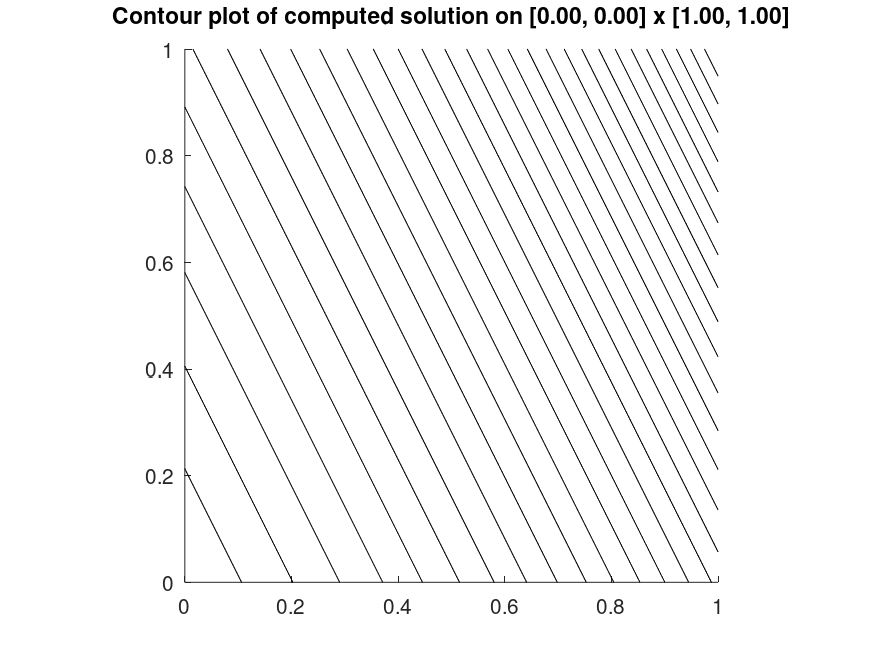
\includegraphics[width=0.5\textwidth]{poisson_5pt_stencil_0-0_1-1_hx-0.003_hy-0.003.png}
        \caption{Contour plot of solution on $[0, 1] \times [0, 1]$ with grid size $\Delta x = \Delta y = 0.0025$}
    \end{figure}
\end{solution}

\pagebreak
b) Modify the script so that it works on a rectangular domain $[a_x, b_x] \times [a_y, b_y]$, but still with
   $\Delta x = \Delta y = h$. Test your modified script on a non-square domain.

\begin{solution}\ \\\\
    We compute relative error for $\Omega = [0, 1] \times [0, 2]$ with step sizes listed below:

    \begin{figure}[h]
        \begin{lstlisting}
        Computed solution on domain [0.00, 1.00] x [0.00, 2.00]: 
 
        Grid points      Grid size (hx, hy)      Relative error
        -------------------------------------------------------
        ( 10,  20)       (0.100000, 0.100000)    3.023e-04 
        ( 20,  40)       (0.050000, 0.050000)    7.654e-05 
        ( 50, 100)       (0.020000, 0.020000)    1.226e-05 
        (100, 200)       (0.010000, 0.010000)    3.065e-06 
        (200, 400)       (0.005000, 0.005000)    7.664e-07 
        (400, 800)       (0.002500, 0.002500)    1.916e-07 
             
        Least squares fit gives E(h) = 0.030209 * h^1.99712
        \end{lstlisting}
        \caption{Output of \texttt{problem\_1b.m} showing decreasing error resulting from grid refinement}
    \end{figure}

    Since our least squares fit for error is given by $E(h) = 0.030209 h^{1.99712}$, we see that the error is 
    $\mathcal{O}(h^2)$, as expected.
    
    \begin{figure}[h]
        \centering
        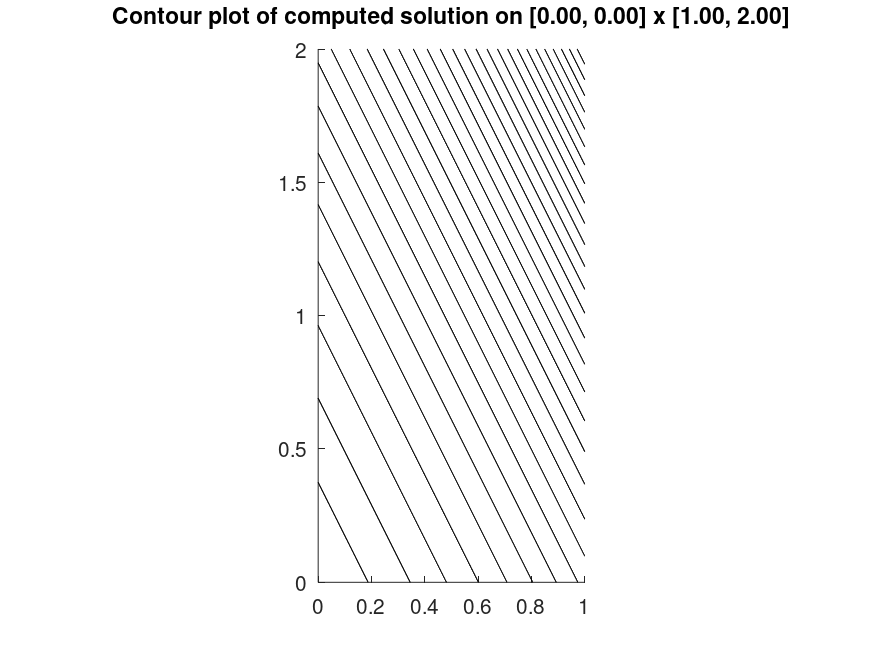
\includegraphics[width=0.6\textwidth]{poisson_5pt_stencil_0-0_1-2_hx-0.003_hy-0.003.png}
        \caption{Contour plot of solution on $[0, 1] \times [0, 2]$ with grid size $\Delta x = \Delta y = 0.0025$}
    \end{figure}
\end{solution}

\pagebreak
c) Further modify the code to allow $\Delta x \neq \Delta y$ and test the modified script.

\begin{solution}\ \\\\
    We compute relative error for $\Omega = [0, 1] \times [0, 2]$ with step sizes listed below:

    \begin{figure}[h]
        \begin{lstlisting}
        Computed solution on domain [0.00, 1.00] x [0.00, 2.00]: 
 
        Grid points      Grid size (hx, hy)      Relative error
        -------------------------------------------------------
        ( 10,  10)       (0.100000, 0.200000)    3.511e-04 
        ( 20,  20)       (0.050000, 0.100000)    8.992e-05 
        ( 50,  50)       (0.020000, 0.040000)    1.441e-05 
        (100, 100)       (0.010000, 0.020000)    3.606e-06 
        (200, 200)       (0.005000, 0.010000)    9.016e-07 
        (400, 400)       (0.002500, 0.005000)    2.254e-07 
             
        Least squares fit in x gives E_x(h) = 0.0350613 * h^1.99446
        Least squares fit in y gives E_y(h) = 0.00879903 * h^1.99446
        \end{lstlisting}
        \caption{Output of \texttt{problem\_1c.m} showing decreasing error resulting from grid refinement}
    \end{figure}

    Since our least squares fit for error with respect to $x$ is given by $E_x(h) = 0.0350613 h^{1.99446}$, and 
    $E_y(h) = 0.00879903 h^{1.99446}$, we see that the error is $\mathcal{O}(h^2)$, as expected.
    
    \begin{figure}[h]
        \centering
        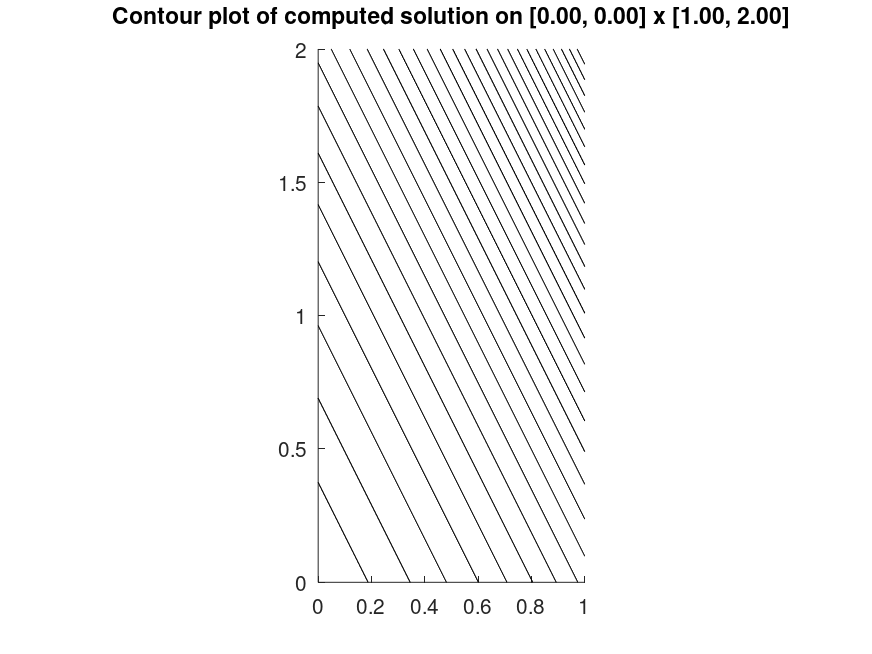
\includegraphics[width=0.6\textwidth]{poisson_5pt_stencil_0-0_1-2_hx-0.003_hy-0.005.png}
        \caption{Contour plot of solution on $[0, 1] \times [0, 2]$ with grid size $\Delta x = 0.0025$ and $\Delta y = 0.005$}
    \end{figure}
\end{solution}